\documentclass[compress,xcolor=table]{beamer}

\usepackage[french]{babel}
\selectlanguage{french}
\usepackage[utf8]{inputenc}
\usepackage[T1]{fontenc}
\usepackage{tikz}
\usepackage{wrapfig}
\usepackage{multirow}
\usepackage{pgf-pie}
\usepackage{pgfplots}
\usepackage{pdfpages}
\usepackage{vocabulaireEpicUnityPresentation}
\usepackage{commun/vocabulaireCommun}
\usepackage{hyperref}
\usepackage{movie15}

\usetheme{eastpic}

% code pour pouvoir mettre des cellcolor qui dépendent de la frame...
\makeatletter
\def\rowcolor{\noalign{\ifnum0=`}\fi\bmr@rowcolor}
\newcommand<>{\bmr@rowcolor}{%
    \alt#1%
	{\global\let\CT@do@color\CT@@do@color\@ifnextchar[\CT@rowa\CT@rowb}% 
	{\ifnum0=`{\fi}\@gooble@rowcolor}% 
}

\newcommand{\@gooble@rowcolor}[2][]{\@gooble@rowcolor@}
\newcommand{\@gooble@rowcolor@}[1][]{\@gooble@rowcolor@@}
\newcommand{\@gooble@rowcolor@@}[1][]{\ignorespaces}
\makeatother



\makeatletter
\def\cellcolor{{\ifnum0=`}\fi\bmr@cellcolor}
\newcommand<>{\bmr@cellcolor}{%
    \alt#1%
	{\global\let\CT@do@color\CT@@do@color\@ifnextchar[\CT@rowa\CT@rowb}%
	 {\ifnum0=`{\fi}\@gooble@cellcolor}%
}

\newcommand{\@gooble@cellcolor}[2][]{\@gooble@cellcolor@}
\newcommand{\@gooble@cellcolor@}[1][]{\@gooble@cellcolor@@}
\newcommand{\@gooble@cellcolor@@}[1][]{\ignorespaces}

\newcommand{\tablenameUn}{Tableau 1 : Temps de conversion en fonction du nombre de fiches}



\def\sectionintoc{}
\def\beamer@sectionintoc#1#2#3#4#5{%
\ifnum\c@tocdepth>0%
\ifnum#4=\beamer@showpartnumber%
{
  \beamer@saveanother%
  \gdef\beamer@todo{}%
  \beamer@slideinframe=#1\relax%
  \expandafter\only\beamer@tocsections{\gdef\beamer@todo{%
      \beamer@tempcount=#5\relax%
      \advance\beamer@tempcount by\beamer@sectionadjust%
      \edef\inserttocsectionnumber{\the\beamer@tempcount}%
      \def\inserttocsection{\hyperlink{Navigation#3}{#2}}%
      \beamer@tocifnothide{\ifnum\c@section=#1\beamer@toc@cs\else\beamer@toc@os\fi}%
      {
        \ifbeamer@pausesections\pause\fi%
        \ifx\beamer@toc@ooss\beamer@hidetext
          \vskip1em
        \else
          \vfill
        \fi
        {%
          \hbox{\vbox{%
              \def\beamer@breakhere{\\}%
              \beamer@tocact{\ifnum\c@section=#1\beamer@toc@cs\else\beamer@toc@os\fi}    {section in toc}}}%
         \par%
        }%
      }%
    }
  }%
  \beamer@restoreanother%
  }
  \beamer@todo%
  \fi\fi%
}



\makeatother
% end code pour pouvoir mettre des cellcolor qui dépendent de la frame


\title{Présentation de projet EDTS - Reconnaissance de parole en utilisant HMM basé sur CMU Sphinx}
\date{\today}
\author{Zhaolun Wang et Zenan Xu}
\institute{\insa}

\setbeameroption{show notes}

\begin{document}


\begin{frame}[plain]
	\titlepage
\end{frame}

\begin{frame}{Sommaire}
	\tableofcontents[hideallsubsections]
\end{frame}

\section[Introduction]{Introduction}
\subsection{}

\begin{frame}{Le client, Fondation UNIT}

\begin{figure}
\centering
\includegraphics[width=5cm]{images/logo.png}
\caption{Logo de la fondation UNIT}
\end{figure}

\begin{itemize}
  \pause
  \item UNIT: l'Université Numérique Ingénierie et Technologie ;
  \pause
  \item Fondation partenariale d'environ 70 Universités, Grandes Ecoles d'Ingénieurs et Entreprises ;
  \pause
  \item Une des sept universités numériques thématiques (UNT) nationales.

\end{itemize}
	
\end{frame}

\begin{frame}{L'équipe \textsc{EpicUnity}}
	
	\begin{figure}
	\centering
	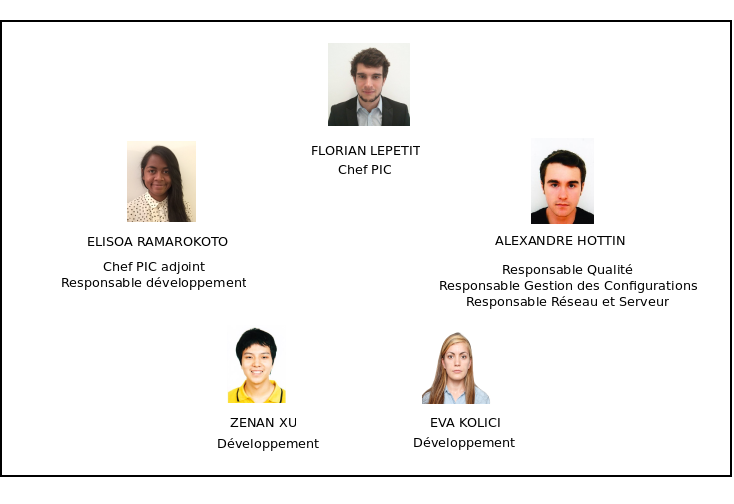
\includegraphics[width=10cm]{images/organigramme.png}
	\caption{Organigramme de l'équipe}
	\end{figure}
	
\end{frame}

\section[Principe de la reconnaissance de la parole]{Modèles acoustiques}
\subsection{}
\begin{frame}{Traitement acoustique : extraction de paramètres}
	\begin{itemize}
	\item MFCC(Mel Frequency Cepstral Coeficients)
	\item LPCC(Linear Predictive Cepstral Coeficients)
	\item PLP(Perceptuqal Linear Predictive analysis)
	\end{itemize}
\end{frame}


\begin{frame}{MFCC}

\begin{figure}
\centering
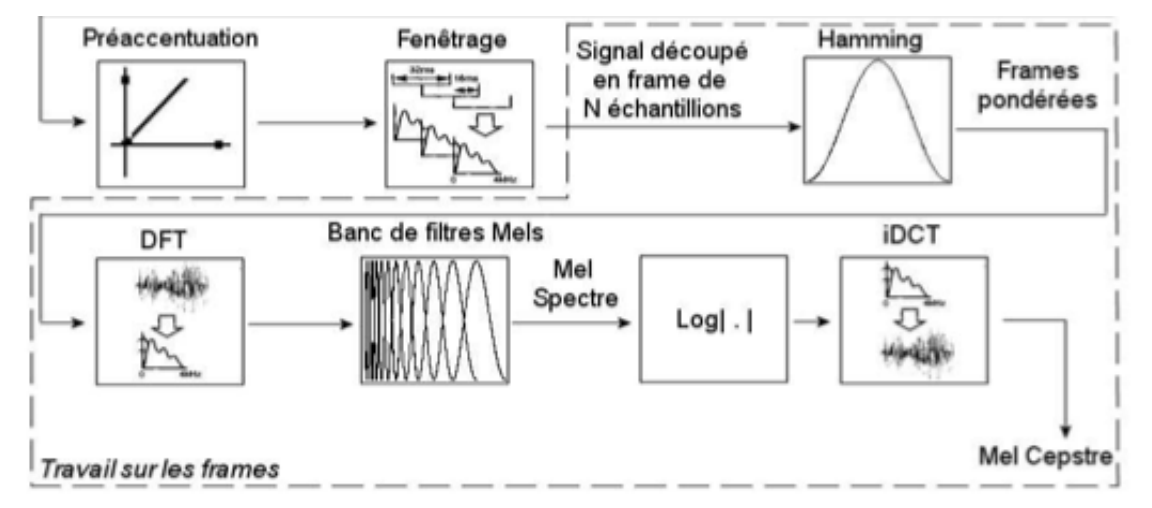
\includegraphics[width=8cm]{images/schema_MFCC.png}
\caption{Schéma de MFCC}
\end{figure}
\end{frame}

\begin{frame}{MFCC}
\begin{itemize}
\item Préaccentuation du signal
\item Découpage du signal en fenêtre
\item Application d’une fenêtre de Hamming
\item Création du banc de filtres
\item Conversion en échelle de mel
\item Application d’une DCT (Discrete Cosinus Transform) sur les portions
\end{itemize}
\end{frame}

\begin{frame}{Décodage acoustique et apprentissage}

\begin{itemize}
\item Chaînes et modèles de Markov cachés  
\item Critère du maximum de vraisemblance
\item Critère de Viterbi
\end{itemize}

\end{frame}

\begin{frame}{Adaptation}
\begin{block}{Méthode MLLR}
La méthode MLLR qui signifie Maximum Likelihood Linear Regression permet d’adapter des modèles acoustiques par régression linéaire.
\end{block}
\begin{block}{Méthode MAP}
La méthode MAP pour estimation du Maximum à postériori est une méthode bayésienne. Elle permet de modifier les paramètres d’un modèle générique pour se rapprocher des données de test.
\end{block}

\end{frame}

\begin{frame}{Création du Modèle acoustique en utilisant Sphinxtrain}
Les données d'entrées sont composés, entre autre:
\begin{itemize}
\item d'un ensemble de fichiers acoustiques(corpus).
\item d'un fichier de transcription qui contient l'ensemble de mots prononcés pour chaque enregistrement(fichier acoustique).
\item d'un fichier qui définie la liste des phonèmes utilisées.
\end{itemize}
\end{frame}

%\section[Principe de la reconnaissance de la parole]{Modèles de langues}
\subsection{}
\begin{frame}{Modèle des N-Grammes}
\begin{figure}
\centering
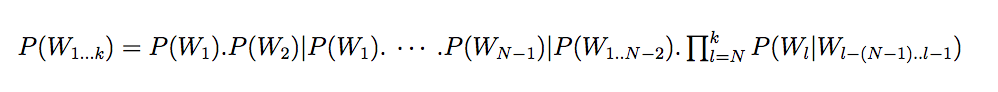
\includegraphics[width=8cm]{images/modele_langage.png}
\end{figure}
\end{frame}

\begin{frame}{Création de Modèle de langage en utilisant CMUCLMTK}
La création d'un Modèle de langage statistique peut se résumer en trois étapes:
\begin{itemize}
\item Collecter des textes
\item Transformer les textes en corpus
\item Transformer le corpus en une distribution de probabilités
\end{itemize}
\end{frame}



\section[Principe de la reconnaissance de la parole]{Modèles de mots}
\subsection{}
\begin{frame}{Modèle des N-Grammes}
\begin{figure}
\centering
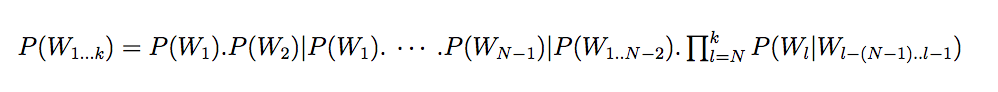
\includegraphics[width=8cm]{images/modele_langage.png}
\end{figure}
\end{frame}

\begin{frame}{Création de Modèle de langage en utilisant CMUCLMTK}
La création d'un Modèle de langage statistique peut se résumer en trois étapes:
\begin{itemize}
\item Collecter des textes
\item Transformer les textes en corpus
\item Transformer le corpus en une distribution de probabilités
\end{itemize}
\end{frame}



\section[Réalisation]{Réalisation du projet}
\subsection{}
%\begin{frame}{Découverte des technologies}

\begin{itemize}
 \item Formation intensive (300 heures-homme);
 \item Acquisition de livres;
 \item Approche par l'exemple;
 \item Appui sur un travail existant : SEMUNIT de Madame Yolaine Bourda.
\end{itemize}

\end{frame}

\begin{frame}{Résultat produit (1/2)}

\begin{itemize}
 \item Un schéma OWL structuré selon le SupLOMFR;
 \item Le vocabulaire SKOS est séparé;
 \item Respect des cardinalités;
 \item Évolutions sur le prochain lot (au niveau de l'inférence).

\end{itemize}
\end{frame}

\begin{frame}{Résultat produit (2/2)}
\begin{itemize}
 \item Des fiches en XML-RDF :
 \begin{itemize}
    \item Issues d'un transformateur opérationnel;
    \item Contenant les triplets RDF d'une fiche;
  \end{itemize}
 \item Vocabulaire externalisé.
\end{itemize}
\end{frame}

\begin{frame}{Garantie de fonctionnement}
\begin{itemize}
 \item Syntaxe, contenu et cohérence;
 \item Compatibilité entre le schéma et la structure des fiches XML;
 \item Une campagne de tests complète.
\end{itemize}
\end{frame}


\begin{frame}{Stratégie de tests}
	\begin{figure}
	  \centering
	  \includegraphics[width=8cm]{images/tests.pdf}
	  \caption{Schéma de principe des tests}
	\end{figure}
\end{frame}

\begin{frame}{Choix des outils de test}

\begin{tiny}
\begin{table}[h]
\begin{tabular}{|c|c|c|c|} \cline{1-4}
Framework & Désordre des triplets & Contenu des balises & \begin{tabular}[c]{@{}c@{}}Bonne formation \\ des triplets\end{tabular}\\ \cline{1-4}
Protégé &  &  & \\ \cline{1-4}
RDFUnit &  &  & \\ \cline{1-4}
XSPEC &  & \checkmark{} & \checkmark{} \\ \cline{1-4}
XSLTUnit &  &  & \checkmark{} \\ \cline{1-4}
Unit testing XSLT &  & \checkmark{} & \checkmark{}\\ \cline{1-4}
\color{red}{Développement par l'équipe} & \color{red}{\checkmark{}} & \color{red}{\checkmark{}} & \color{red}{\checkmark{}} \\ \cline{1-4}
\end{tabular}
\end{table}
\end{tiny}

\begin{itemize}
 \item Des solutions développées par l'équipe;
 \item XML-RDF : xmllint + Python (basé sur rdflib);
 \item OWL : W3C, vérifications manuelles et un raisonneur.
\end{itemize}

\end{frame}


\begin{frame}{Volumétrie}

\begin{figure}
    \centering
    \includegraphics[width=7cm]{images/volumetrie.pdf}
    \caption{Transformation de fiches distinctes}
\begin{tiny}
\begin{table}[h]
\begin{tabular}{|c|c|c|c|c|c|c|c|c|}
\cline{1-9}
nombre de fiches & 1 & 2 & 10 & 50 & 100 & 500 & 1000 & 5000\\ \cline{1-9}
temps de conversion (s) & 1,14 & 2,3 & 11,68 & 58,04 & 116,21 & 579,63 & 1158,89 & 5794,56 \\ \cline{1-9}
\end{tabular}
\end{table}
\end{tiny}
\tablenameUn{}
  \end{figure}

\end{frame}

\begin{frame}{Démonstration}

Démonstration de requêtes SPARQL.
\centering
\includemovie[controls,poster]{6cm}{6cm}{video/demo.mp4}

\end{frame}


\section[Amélioration]{Amélioration}
\subsection{}

\section[Conclusion]{Conclusion}
\subsection{}

%\begin{frame}{Conclusion}
	\begin{itemize}
	\item Démarche enrichissante :
		\begin{itemize}
			\item Développement en méthodes de type agile;
			\item Démarche Qualité.
		\end{itemize}
		\vspace{0.2cm}
	\item Sujet passionnant :
		\begin{itemize}
			\item Découverte web sémantique ;
			\item Formation et perfectionnement dans différents domaines;
			\item Démarche de R\&D novatrice dans le domaine.
		\end{itemize}		
	\item Vers l'inférence et la gestion des personnes.
	\end{itemize}
\end{frame}

\end{document}






